% Supplementary Information for:
% Simplex Constraints, Spatial Generalization, and the Regressor--Detector
% Gap in Machine-Learning Surrogates for CALPHAD Phase-Fraction Prediction.
%
% This supplement accompanies the main manuscript. Section, table and
% figure numbers here carry an S prefix (Section S1, Table S1,
% Figure S1, ...). All numbered values are generated from the same stored
% result artefacts as the main text (paper/tables.py, paper/figures.py);
% nothing is hand-entered.
\documentclass[11pt,a4paper]{article}
\usepackage{amsmath,amssymb}
\usepackage{graphicx}
\usepackage{booktabs}
\usepackage[authoryear,round]{natbib}
\usepackage[colorlinks=true,linkcolor=blue,citecolor=blue,urlcolor=blue]{hyperref}
\setlength{\textwidth}{16cm}
\setlength{\textheight}{23cm}
\setlength{\oddsidemargin}{0cm}
\setlength{\evensidemargin}{0cm}
\setlength{\topmargin}{-1cm}

\begin{document}

\begin{center}
{\Large Supplementary Information} \\[1ex]
{\large Simplex Constraints, Spatial Generalization, and the
Regressor--Detector Gap in Machine-Learning Surrogates \\
for CALPHAD Phase-Fraction Prediction} \\[1ex]
Anonymous
\end{center}

% ======================================================================
\section{Failed constraint mechanisms in full}
\label{sec:si-negative}

Three constraint mechanisms that are plausible in principle fail in
practice under the evaluated protocol. The main text
(Section~4 there) summarises each as a scope delimiter; the full
evidence follows here.

\subsection{Sparsemax: severe seed sensitivity under the evaluated
configuration}

Sparsemax \citep{martins2016sparsemax} projects the logits onto the simplex,
producing exact zeros for phases the model deems absent. It satisfies closure
to $\le 5\times10^{-8}$ and achieves the sparsity that softmax cannot. But
under the evaluated training configuration it exhibited severe seed
sensitivity and substantially worse MAE than the other constrained heads:
2--4 times worse than renorm or sigmoid/$\Sigma$, with the three seeds
giving 0.018/0.037/0.117 on Fe--Cr--Mo, 0.053/0.067/0.013 on Fe--Cr--Ni,
and 0.019/0.015/0.079 on Fe--Mn--Ni --- a seed standard deviation of the
same order as the mean (Figure~\ref{fig:si-failures}, panel a).

The observed behaviour is consistent with a \emph{sparsity trap}: once the
sparsemax projection drives a phase's logit below the threshold $\tau$,
the gradient at that logit is exactly zero, so a phase that starts out
clipped can never recover, and whether it recovers is decided by
initialisation. We present this as a mechanistic interpretation of the
observed seed sensitivity, not as a demonstrated cause; the experiment
evaluates one implementation and optimisation configuration. Notably, the
head was trained with a regression loss on its projected outputs --- the
configuration most exposed to that zero-gradient region --- so the
dedicated sparsemax loss and $\alpha$-entmax variants remain untested; a
fixed-scale entmax ($\alpha < 2$) or a warm start from softmax would be the
natural remedies. We therefore do not claim that sparsemax is
unsuitable for phase-fraction prediction in general --- only that it
performed poorly and unreliably under the configuration studied here.

\subsection{Sum-to-one penalty: redundant and harmful}

The penalty head of the main text (ablation study) is included here as a
negative result. The sum-to-one constraint is already satisfied by the
targets; adding it as a soft penalty creates a redundant loss term that
competes with the data fit. At $\lambda = 10$ the penalty dominates the Huber
loss entirely, and the model learns to minimise closure violation at the
expense of phase-fraction accuracy.

\subsection{Residue closure: closure without non-negativity, and the
error concentrates}

The residue head predicts $K{-}1$ phase fractions and closes the sum
algebraically: $\hat y_K = 1 - \sum_{k<K} \hat y_k$. This enforces the
sum-to-one equality by construction but does not intrinsically guarantee
non-negativity: if the other predicted fractions sum to more than one, the
residue is negative. In the stored predictions the residue head emits
negative values on 0.0\% (Fe--Cr--V), 0.02\% (Fe--Mn--Ni), 0.40\%
(Fe--Cr--Ni), 0.50\% (Fe--Cr--Mn), and 1.21\% (Fe--Cr--Mo) of cells, with
the most negative cell at $-0.59$. It is therefore closure-valid but not
simplex-valid, and any deployment would need a projection step after all.

Beyond admissibility, the head is also the least accurate constrained
variant: even the best residue head is 1.4--2.5 times worse than the best
constrained head in the same system, and the choice of which phase to drop
matters --- a sweep over all $K$ choices (Figure~\ref{fig:si-failures}, panel
c) shows the best choice is the dominant phase in four of the five ternary systems. The
observed degradation is consistent with the residual phase absorbing the
accumulated prediction error of the other $K{-}1$ channels; we note this
as an interpretation supported by the sweep, not a directly demonstrated
mechanism.

\begin{figure}[htbp]
\centering
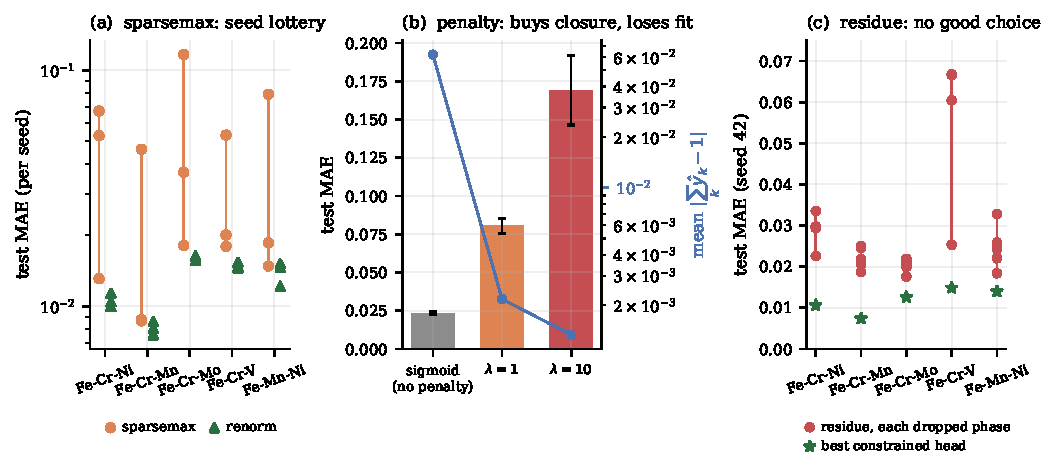
\includegraphics[width=\textwidth]{figures/fig6_failures}
\caption{Three negative results. (a) Sparsemax: per-seed test MAE (orange)
versus the renorm head (green) across all five ternary systems. The seed-to-seed
spread of sparsemax is of the same order as its mean. (b) Sum-to-one penalty
on Fe--Cr--Ni: MAE (bars, left axis) and closure violation (line, right axis)
as $\lambda$ increases. The penalty buys closure at the cost of the fit.
(c) Residue sweep: per-phase MAE for each choice of dropped phase (red)
versus the best constrained head (green star) across all five ternary systems.}
\label{fig:si-failures}
\end{figure}

% ======================================================================
\begin{thebibliography}{99}

\bibitem[Martins and Astudillo(2016)]{martins2016sparsemax}
Martins, A.F.T., Astudillo, R.F., 2016. From softmax to sparsemax: A sparse
model of attention and multi-label classification. Proc.\ ICML, 1614--1623.

\end{thebibliography}

\end{document}
